\documentclass[conference,a4paper]{IEEEtran}
% Supplementary material for AMICT 2026 submission.
\usepackage{cite}
\usepackage{url}
\usepackage{graphicx}
\usepackage{amsmath}
\usepackage{booktabs}
\usepackage{microtype}

\title{Supplementary Material:\\
Content-Conditioned Cyclic Seam Carving for Equirectangular Panoramas}

\author{\IEEEauthorblockN{Anonymous Authors}
\IEEEauthorblockA{Affiliation withheld for double-blind review}}

\begin{document}
\maketitle

\begin{abstract}
This supplement holds extended protocol, extra analysis, and
additional body-column stills. The method overview, polar
scatter, head/body examples, temporal control, and four-stem
qualitative panel appear in the main paper. Locked experimental
numbers in the main text are unchanged here. Code and remaining
data will be attached with this file.
\end{abstract}

\begin{IEEEkeywords}
equirectangular panorama, seam carving, supplementary material
\end{IEEEkeywords}

\section{Code and Remaining Data}
\label{sec:supp-code}

The following will be included with this supplement (not yet
packed in this PDF):
\begin{itemize}
  \item Source code for cyclic seam routing, spherical energy
  $E_p=E_g\cos\phi$, the content-conditioned gate
  ($\tau=0.20$, $k=24$), and the SegFormer-B0 ADE20K person-map
  wrapper.
  \item Configuration files and scripts that reproduce Tables~I--III
  of the main paper at width at most $512$.
  \item Remaining evaluation outputs (per-image hit rates, gate
  ON/OFF flags, temporal photometric residuals) that do not fit
  in the main text.
\end{itemize}
PanoCount stills and head-point annotations follow
the collection cited in the main paper~\cite{arbi2025panocount}.
That counting paper is accepted at {PRICAI} 2026; the
implementation is public at
\url{https://github.com/aiguo112/PanoCount360}. The stills used
in the carving experiments are not treated as a public
downloadable benchmark; dataset access follows the request
process of that repository.

\section{Extended Experimental Protocol}
\label{sec:supp-protocol}

Polar band means the top and bottom $15\%$ of rows.

\textbf{Occupancy.}
Fraction of seam pixels whose row lies in the polar band.
Any vertical seam occupies that band at a rate fixed by the band
height (here $0.297$). Occupancy is a sanity check, not the
spherical outcome.

\textbf{Routing share.}
Fraction of cyclic $|\Delta x|$ whose starting row is in the
polar band. A wrap step counts as $1$\,px using the seam's own
width. Mean polar $|\Delta x|$ is the mean cyclic step on
polar-band rows, in pixels.

\textbf{Head-hit rate.}
A GT head is hit if any of the first $k$ original-width seams,
on that head's row, satisfies cyclic
$|x-x_{\mathrm{head}}|\le r(\phi)$, with
\begin{equation}
r(\phi)=\frac{r_{\mathrm{eq}}}{\max\bigl(|\cos\phi|,\cos 75^\circ\bigr)},
\quad
r_{\mathrm{eq}}=W\cdot\frac{2^\circ}{360}.
\end{equation}
Reported as a percentage of GT heads.

\textbf{Body-hit rate.}
A GT person is hit if any of the first $k$ original-width seams
cuts that person's constructed body column: a meridian strip from
the head downward by $12^\circ$ of latitude, half-width
$2.5\,r(\phi)$. Reported as a percentage of GT persons. Body-hit
is not head-hit and is not a segmentation IoU.

\textbf{Predicted-person instance hit rate.}
A SegFormer-B0~\cite{xie2021segformer} model trained on
{ADE20K}~\cite{zhou2017ade20k}
(\texttt{nvidia/segformer-b0-finetuned-ade-512-512}) predicts a
per-pixel class map. The person class is selected by label name;
there is no logit threshold beyond $\mathrm{argmax}$. Instances
are eight-connected components of that binary map with no minimum
size. Components are computed on the planar $H\times W$ grid and
do not wrap across $x=0$ and $x=W-1$. The metric is the fraction
of those instances touched by any of the first $k$ original-width
(b) seams.

\textbf{Gate.}
Let $h_{\mathrm{pred}}$ be that fraction for $k=24$. If there are
no predicted-person instances, $h_{\mathrm{pred}}=0$ and the gate
is off. When the gate is on, (c) is used ($\lambda_s=4$ on the
predicted $0/1$ person map); when it is off, (b) is kept. Both
seam sets are always computed from the original image; the gate
only selects which set is the method output. This instantiation
is not equivalent to the oracle that paints GT body columns.

\textbf{Temporal photometric validation.}
Equatorial phase correlation~\cite{reddy1996fft} estimates a
cyclic horizontal pan; the polar $15\%$ of rows is excluded.
Photometric residual is measured on the same equatorial band,
before and after warping $I_t$ by the estimated pan. Post-warp
photometry, not pan magnitude, is the test of whether the
estimate reflects camera motion.

\textbf{Statistics.}
The $95\%$ CI in the main paper is the paired
normal-approximation interval on $n=171$ images. Many per-image
differences are exactly zero, including all gate-off images. The
mean is the paired average on the pre-specified medium split; it
is not a typical per-image effect, and no multiple-testing
correction is applied. The practical SegFormer run was executed
after the oracle GT analysis and is not a pre-registered
hypothesis test of the gate.

\section{RQ1 Scatter}
\label{sec:supp-c1}

The corresponding scatter is in the main paper. On CVRG-Pano
val+test ($n=120$), the pre-registered content
predictor---unweighted polar/equator Sobel mean, range
$0.14$--$0.74$---does not track polar routing $\Delta$. Every
image has polar Sobel mean below the equatorial mean
(ratio $<1$). Spherical energy therefore remains a legal term.
On this corpus it is a small routing effect, not a large polar
detour, and it is not explained by polar texture.

\section{Head-Disk Qualitative Example}
\label{sec:supp-head}

The largest medium head-hit pair is in the main paper
(panels (a)--(b) of the combined example figure).

Among the $84$ medium images where (b) hits at least one head,
$82/84$ go down under always-on head-disk energy. The other $87$
are $0\to 0$ ties. Scene composition---thin seams versus clustered
$2^\circ$ disks---leaves little head-cut to undo.

\section{Oracle Body-Column Examples}
\label{sec:supp-body}

The largest oracle high-body pair is in the main paper
(panels (c)--(d) of the combined example figure). Magenta there
is constructed GT body columns. Fig.~\ref{fig:supp-extra-body}
shows three further medium stills under the same overlay
convention.

\begin{figure*}[t]
  \centering
  \begin{minipage}[t]{0.32\linewidth}
    \centering
    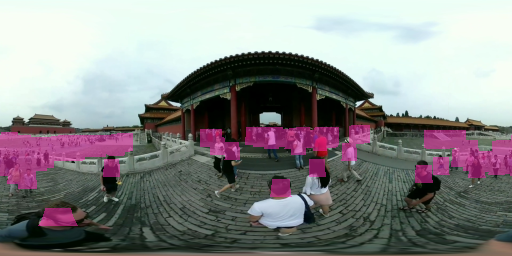
\includegraphics[width=\linewidth]{figures/fig_body_149.png}\\
    {\small (a) Stem $149$}
  \end{minipage}\hfill
  \begin{minipage}[t]{0.32\linewidth}
    \centering
    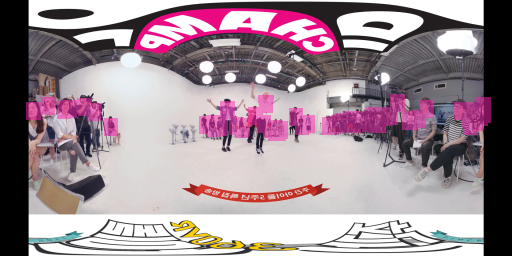
\includegraphics[width=\linewidth]{figures/fig_body_166.png}\\
    {\small (b) Stem $166$}
  \end{minipage}\hfill
  \begin{minipage}[t]{0.32\linewidth}
    \centering
    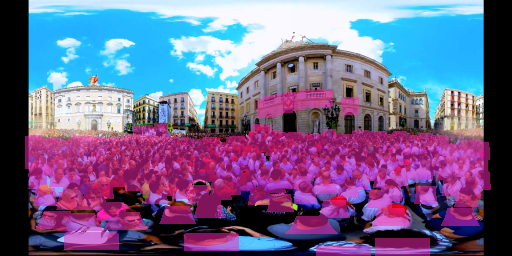
\includegraphics[width=\linewidth]{figures/fig_body_729.png}\\
    {\small (c) Stem $729$}
  \end{minipage}
  \caption{Additional PanoCount medium stills with constructed GT
  body columns (magenta) and spherical baseline seams (red).
  These frames are extra illustrations; they are not the largest
  oracle high-body case used in the main paper.}
  \label{fig:supp-extra-body}
\end{figure*}

On the oracle high-body subset, (c) uses essentially all of the
baseline damage. On the complement, (b) already hits $3.4\%$ of
columns. The all-medium oracle mean is the $49$-image tail.
Body columns remain a constructed proxy (near-field boxes are
mostly head and shoulders; dense crowds merge).

\section{Why Conditional Protection?}
\label{sec:supp-why}

The practical gate changes the seam set on $56/171$ medium
images. The other $115$ keep the spherical baseline. The
all-medium $-1.55$\,pp is therefore a mixture: a nonzero paired
change on the selected subset ($-4.73$\,pp) and a structural
zero on the rest. On the selected subset the GT sign is mixed
($34$ down, $5$ tied, $17$ up), so the ON mean is not a claim
that every activation helps on GT columns. The experiment
describes where $\lambda_s$ has work to do. It does not show
that $\tau=0.20$ is optimal, or that the gate is better than
other simple rules a practitioner might try after seeing the
same regime split. Gain is concentrated where predicted baseline
risk is at least $\tau$, which is the regime the rule was
designed to isolate. That pattern is consistent with semantic
protection being regime-dependent on this split. It is not a
causal claim that $\tau=0.20$ is optimal, nor that SegFormer
person pixels cause the GT reduction: the gate is a selection
rule, and GT body-hit is a held-out score of a different object.

The same concentration appears in the oracle table, at a
different scale and with a different detector. High-body GT
columns give $-35.2$\,pp on $49$ images and $-3.4$\,pp on $122$.
The practical ON set ($n=56$) overlaps that oracle subset on
only $30$ images ($19$ high-body images remain gate-OFF).
Predicted-person instances are not GT bodies, and $-4.73$\,pp is
not $-35.2$\,pp. Conditional use of $\lambda_s$ is supported as
a description of where the energy has work to do, not as
equivalence of the two gates.

\section{Temporal Control}
\label{sec:supp-temporal}

Temporal compensation is not part of the proposed carving
pipeline. This section is a control on the camera-motion
assumption a compensated-frame method would need.

The control fixes one real ERP frame $I_t$ (clip ERP2, source
$1626$, width $512$).

\begin{enumerate}
  \item[(A)] \textbf{Known cyclic yaw.}
  Rolling the full ERP by $k\in\{8,16,32,64,128,141\}$ pixels,
  the estimator recovers each $k$ exactly and the post-warp
  photometric residual is zero. Phase correlation is correct on
  this projection when the motion is a genuine yaw.

  \item[(B)] \textbf{True consecutive frame} ($\Delta t=0.03$\,s).
  Estimated pan $0.00$\,px; equatorial dense-flow $u$ $0.00$\,px.
  Warping does not change the residual (ratio $1.00$). At video
  rate there is no motion to regularize, and the estimator
  introduces none.

  \item[(C)] \textbf{Linspace neighbor}
  ($\Delta t=7.74$\,s; $232$ frames).
  The estimator returns $253$\,px on the worst pair (clip-mean
  absolute pan $141$\,px). Warping $I_t$ by that shift leaves
  the equator essentially unchanged: residual falls only to
  $0.95$ of raw ($56.2\rightarrow 53.5$).
\end{enumerate}

A warp that explained camera motion would drive the residual
toward zero, as in (A). Condition (C) does not, so the $253$\,px
shift does not account for the sparse neighbor. Consecutive-frame
windows of ERP2, ERP4, and ERP5 in this corpus agree near zero;
we found no validated video-rate yaw window. This is not a test
of whether temporal seam propagation works when genuine
inter-frame yaw is present, and it is not offered as a successful
temporal method.

The three-condition control figure is in the main paper; this
section keeps the per-condition protocol.

\section{Qualitative Notes}
\label{sec:supp-qual}

In every main-paper qualitative panel the magenta overlay is
SegFormer predicted person pixels, not GT. GT body-hit in the
caption is the evaluation score, not the gate statistic
$h_{\mathrm{pred}}$.

Stem $166$ is gate OFF: predicted instance hit is $0$, GT
body-hit is $0$, and the output equals (b). Stem $242$ is also
gate OFF ($h_{\mathrm{pred}}=0$) but GT body-hit is $16.9\%$:
predicted components miss people that the GT columns still
count, so the gate leaves residual GT damage untouched. Stem
$800$ is gate ON and a successful protection case on the GT
score ($26.7\%\rightarrow 15.5\%$), one of the $34/56$ ON images
where GT body-hit falls; this image is also in the oracle
high-body set, which we note as overlap, not as proof that the
practical detector found GT columns. Stem $915$ is gate ON with
the opposite GT movement ($11.7\%\rightarrow 22.3\%$), one of
the $17/56$ ON images where predicted-person energy increases GT
body-hit when the two person representations disagree. These
frames illustrate operating regimes. They are not a random
sample and are not a performance claim.

\bibliographystyle{IEEEtran}
\bibliography{IEEEabrv,refs}

\end{document}
